% Chapter Template

\part {Search for heavy neutral leptons}


\chapter{Heavy Neutral Leptons} 
\label{Chapter3} 


In the SM, all the fermions are known to have both left- and right-handed chirality, the only exception comes from the neutrinos.

The recent neutrino oscillation experiments have clearly and
definitely shown that neutrinos are massive.

The light masses of the SM neutrinos ($\nu_{SM}$) can be explained by introducing massive right-handed neutrinos ($\nu_{R}$), often referred to as \emph{heavy neutral leptons} (HNLs), via a type-I seesaw mechanism~\cite{MINKOWSKI1977421,gellmann2013complex,PhysRevLett.44.912,PhysRevD.22.2227}.
Another possible indication comes from the possibility to consider
$\nu_{R}$ as part of the explanation for the baryon asymmetry of the
universe; the $\nu_{R}$ mixing violates \emph{CP} symmetry and the $\nu_{R}$ interaction may potentially generate a matter-antimatter asymmetry in the early stage of the formation of the universe~\cite{Canetti_2012,KUZMIN198536}.

These few examples, which are going to be explored later on, already
show the relevance and the interest for the HNL search program, and
provide strong motivations to investigate the existence of the
$\nu_{R}$. This huge enthusiasm has led in the past $\sim10$ years to
the creation of a very active community with strong synergy between
theorists and experimental collaborations. It had contribute to the publication of an impressive numbers of papers and the proposal of a considerable number of experiments focused mainly on heavy neutral leptons. 

\section{Neutrino Portal} \label{sec:neutrinoPortal}
The \emph{neutrino portal} is defined as the coupling of one or more dark fermions $N_{I}$  ($I = 1,2,...$ $\mathcal{N}$), which are sterile with respect to the SM gauge interactions, to the gauge-invariant operator $\bar{L}_{\alpha}  \cdot \widetilde \Phi$; the general form of the neutrino portal could be written as: 
\begin{equation}
\label{eq:neutrinoportal}
\mathcal{L} = \mathcal{L}_{SM} + \mathcal{L}_{DS} + \sum F_{\alpha I} (\bar{L}_{\alpha}  \cdot \widetilde \Phi)N_{I} + h.c.
\end{equation}

where the summation loops over the flavor of lepton doublets
${L}_{\alpha}$ ($\alpha = e,\; \mu, \: \tau$) and the number of
available HNLs $N_{I}$; $F_{\alpha I} $ are the Yukawa couplings and
$\Phi$ is the Higgs doublet. The term $\mathcal{L}_{DS}$ is the dark
sector lagrangian which contains the mass term of HNLs which can be
either of Majorana or Dirac nature~\cite{Alekhin_2016}.
Fixing the $\Phi$ to its vacuum expectation value, $\widetilde \Phi = \frac{1}{\sqrt{2}} \binom{v}{0}$, and diagonalizing the mass term of the dark fermions, the last term in Eq.~\ref{eq:neutrinoportal} brings to the quadratic mixing of the neutrinos $\nu_{\alpha}$ with the $N_{I}$; this mixing is parametrized by a matrix $V$. In the minimal HNL models, the elements of the matrix $V$ control both the production and the decay of the HNLs. 
If $\mathcal{N} = 3$, there is a right-chiral counterpart for each $\nu_{SM}$, see fig.~\ref{fig:c3sm_extension}. The fermion $N_I$ can have mass $M_I$, which is independent  of the value of $F_{\alpha I}$.
\begin{figure}[t!]
  \centering
  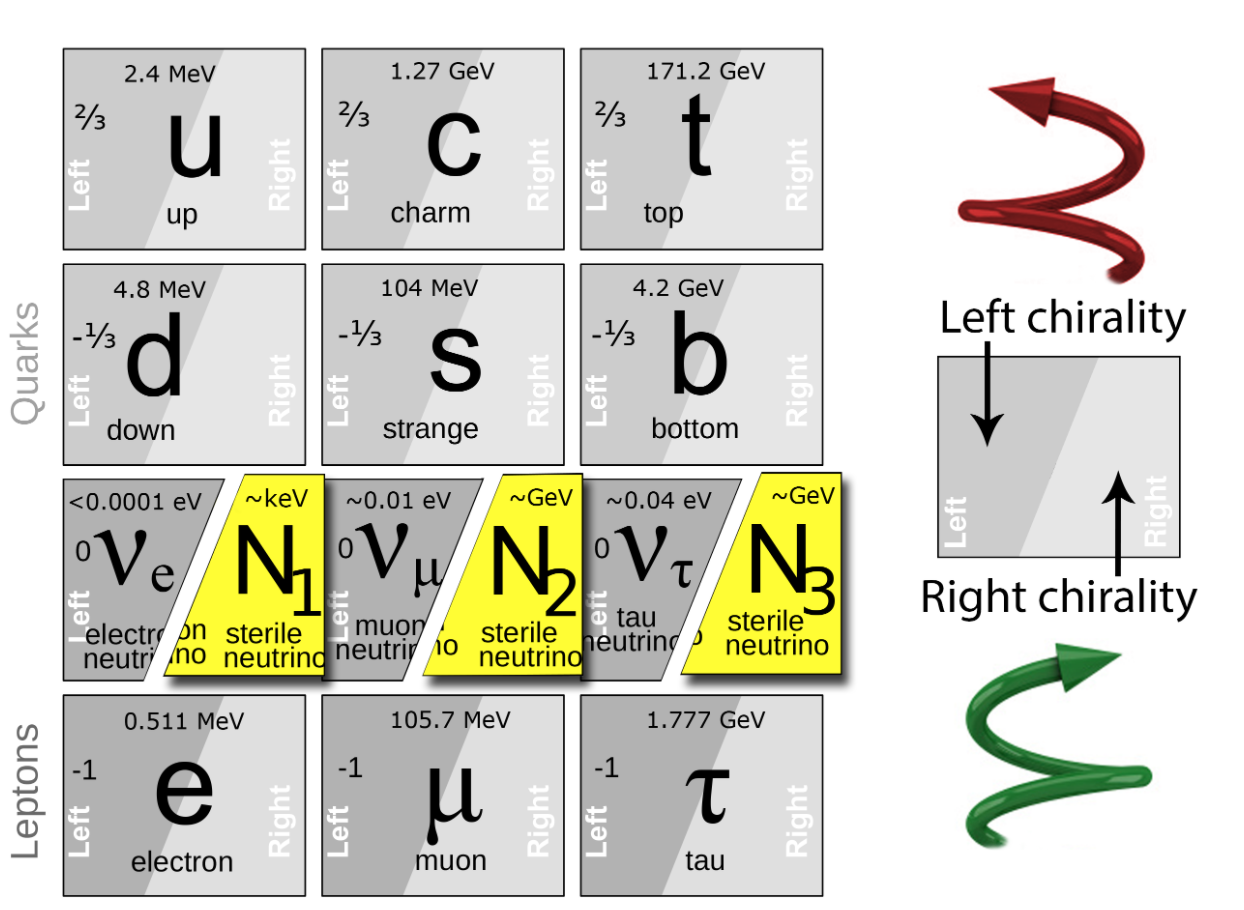
\includegraphics[width=.60\textwidth]{Figures/c3/SM_extension}
    \caption{There are 3 SM neutrinos $\nu_{e}, \; \nu_{\mu}, \;\nu_{\tau}$ which are massless and always left-chiral; 3 right-chiral counterparts are added $N_{1}, \; N_{2}, \;N_{3}$. They are sterile so they do not feel the electric, weak and strong forces. However they can be produced through mixing with the $\nu_{SM}$ with the corresponding mixing parameter.}
  \label{fig:c3sm_extension}
\end{figure}

Many HNL models require the existence of two or more right-handed neutrinos. In experimental searches, however, following a model-independent approach, we can consider the production of a \emph{single} HNL, which be light enough to be kinematically accessible at the accelerator experiments; see the full overview in~\cite{Atre_2009}. 

Under this assumption, there are then only two free parameters to be
constrained: the mass $M_I$ of the HNL and its mixing parameter with
the SM neutrino of flavor $\alpha$, controlled by the Yukawa coupling
$F_{\alpha I}$. The experimental sensitivity is expressed in terms of
the coupling $|V_{\alpha I}|^2$ ($= |F_{\alpha I}|^2$) as a function
of $M_I$ for a given flavor $\alpha$. It is frequently assumed that in
the matrix $V$ the other mixing elements for the residual flavors are
zero; although it does not translate into a valid concrete model, this latter consideration it is very useful to evaluate the experimental sensitivity on the single $|V_{\alpha I}|^2$ without involving any model dependent hierarchy between the different flavor mixings. 
%\begin{figure}[h]
%  \centering
%  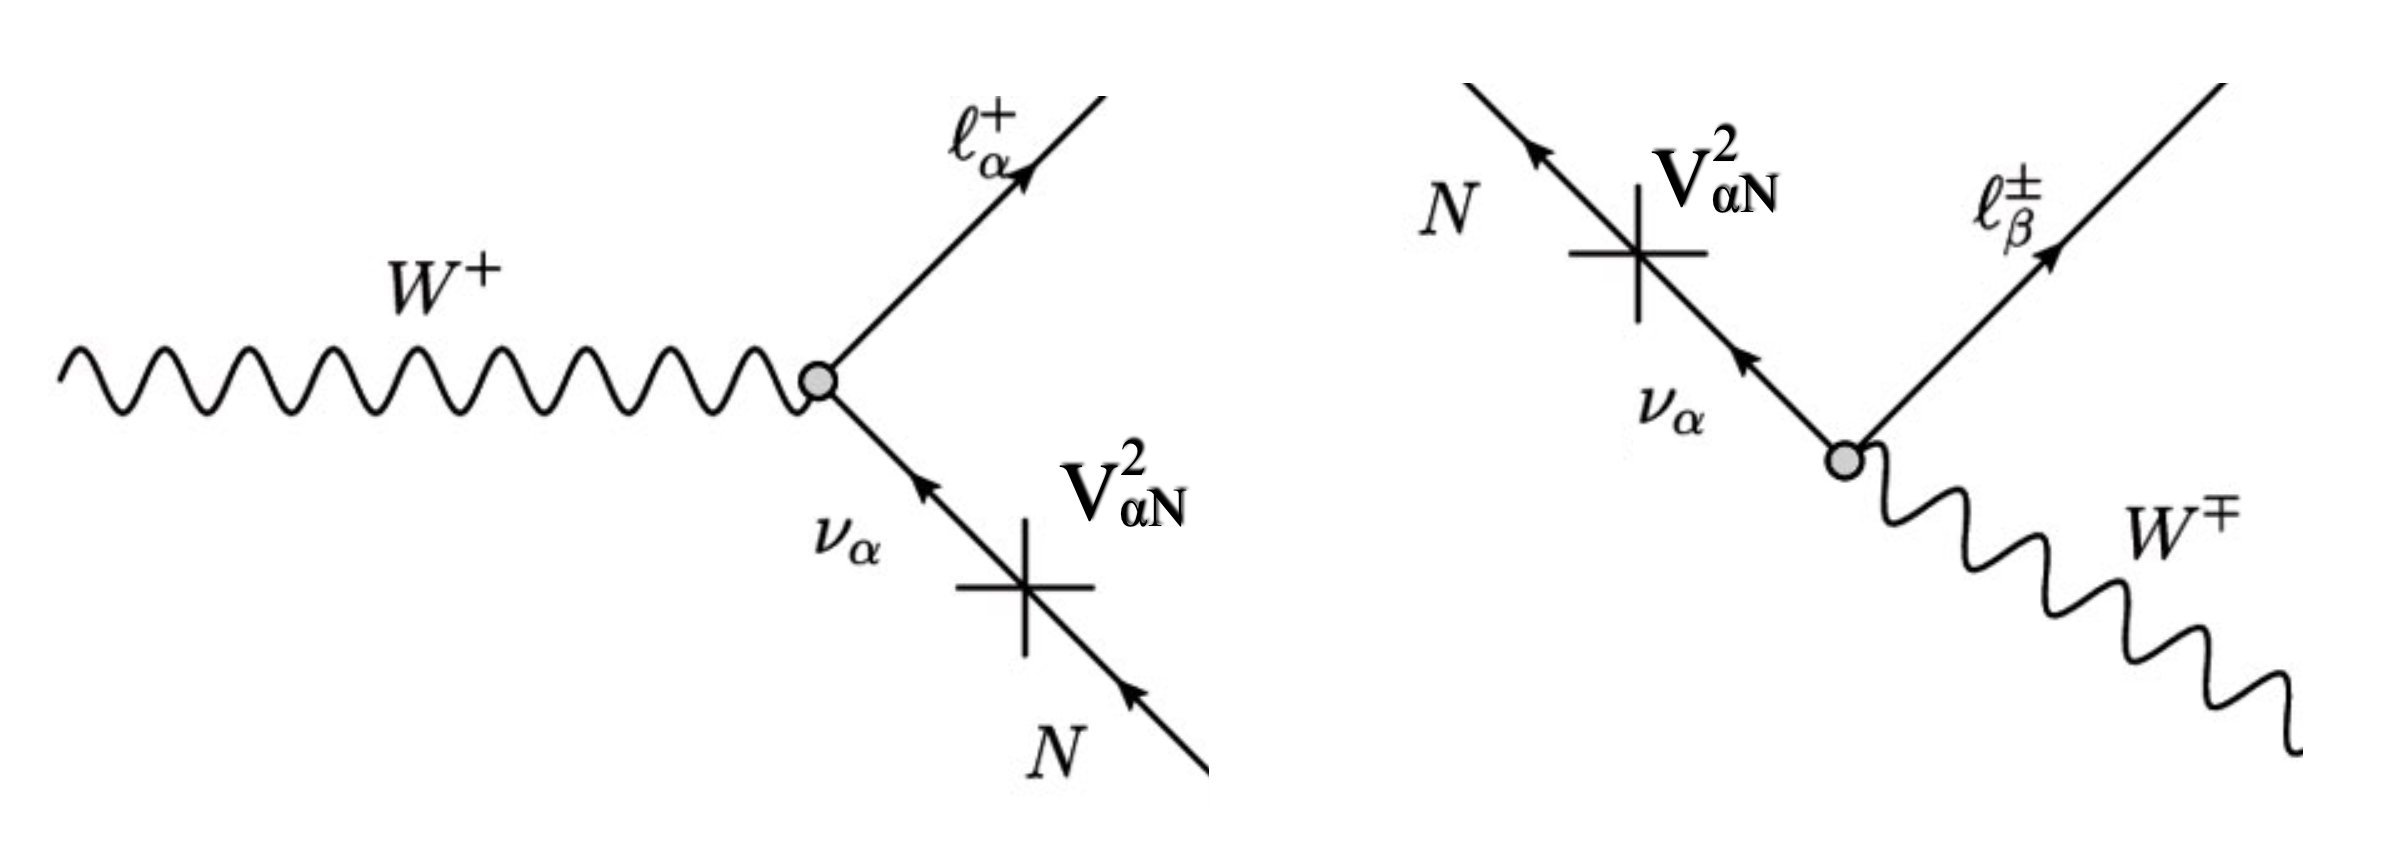
\includegraphics[width=.80\textwidth]{Figures/c3/diagram_decay}
%    \caption{Production (left) and decay (right) of the particle $N_{I}$.}
%  \label{fig:c3diagram_decay}
%\end{figure}

\section{Heavy neutral lepton formalism and extension of the standard model}
To set up our notation and conventions, we first discuss the formalism for the simplest
extension of the SM that includes right handed singlets. In section~\ref{sec:currentlimits}, we will try to contextualize the theory, explained here, summarizing the current constraints on the mass and mixing of a heavy neutrino from various direct
detection experiments, accelerator searches and electroweak precision
fits.

\subsection{Seesaw mechanism}\label{sec:seesaw}
The most general renormalizable Lagrangian for the neutrino masses includes both the Dirac and Majorana mass terms. The SM Lagrangian $\mathcal{L}_{SM}$ is extended adding $\mathcal{N}$ right-handed neutrinos $N_I$ (for notations see Eq.~\ref{eq:neutrinoportal}):
\begin{equation}
\label{eq:fullSMLag}
 \mathcal{L} = \mathcal{L}_{SM}+ i \bar N_I \partial_\mu \gamma^\mu N_I -
  \left(F_{\alpha I} \,\bar L_\alpha N_Is \tilde \phi 
    - \frac{M_I}{2} \; \bar {N_I^c} N_I + h.c.\right)
\end{equation}
As already explained in the section~\ref{sec:neutrinoPortal}, these $N_I$ are neutral with respect to all the gauge interactions of the SM, thus are called \emph{sterile neutrinos} or \emph{gauge-singlet fermions}.
In the Higgs phase, the term~\ref{eq:neutrinoportal} brings to the $\nu_{\alpha} - N_I$ mixing. As a result the \emph{charge eigenstates} of $\mathcal{L}_{SM}$ (Eq.~\ref{eq:fullSMLag}) do not coincide with \emph{mass eigenstates}, which can be extracted by diagonalizing the following matrix:
\begin{equation}
\label{eq:matrixmass}
 \mathcal{M}_{\nu,N} = 
\begin{pmatrix}
0 & m_D\\
m^{T}_{D} & M_I
\end{pmatrix}
\end{equation}
with the matrix elements defined as: $m_D = 3 \times  \mathcal{N}$ Dirac mass matrix, $(m_D)_{\alpha I} = F_{\alpha I}v, \; v = \sqrt{2}\langle \Phi \rangle$ and $M_I$ is $\mathcal{N} \times \mathcal{N}$ matrix of Majorana masses.

Considering the relation between $M_I$ and $m_D$, we could explore two interesting extreme limits:
\paragraph {Pure Majorana neutrino, $m_D \ll M_I$.}
In this limit, the mass matrix gives rise to 3 almost pure right-handed neutrinos with heavy Majorana mass $M_I$ and 3 almost pure left-handed neutrinos with light Majorna mass $m_\nu = - (vm_D)^{T}M^{-1}_{I}(vm_D)$ which are the 3 eigenvalues of the matrix $(\mathcal{M}_{\nu})_{\alpha \beta}$. This mechanism is then referred to as the \emph{seesaw mechanism}\footnote{This mechanism is usually called \emph{Type-I seesaw}. \emph{Type-II seesaw} has an extra SU(2) triplet scalar~\cite{Deppisch_2015}; in \emph{Type-III seesaw} an extra fermion in the adjoint of SU(2) is added to the model~\cite{Foot:1988aq}}~\cite{MINKOWSKI1977421}~\cite{Mohapatra:1979ia}~\cite{Yanagida:1979as}.
\begin{figure}[h]
  \centering
  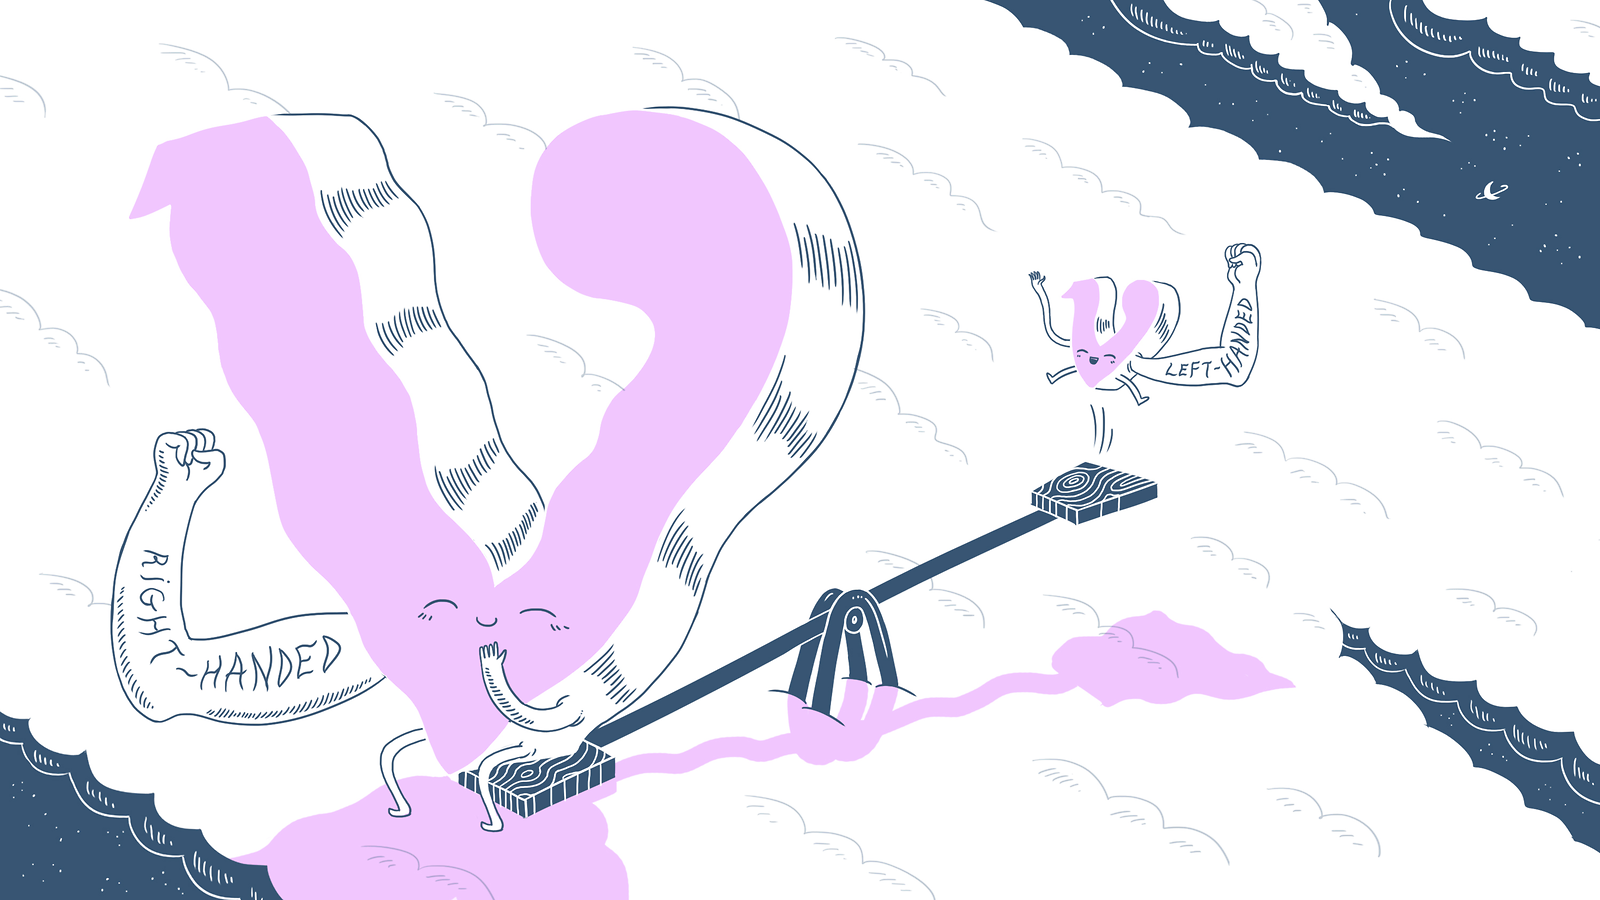
\includegraphics[width=.60\textwidth]{Figures/c3/funny.png}
    \caption{Silly representation of the \emph{seesaw mechanism}~\cite{funny}. Note that for a fixed value of $m_D$, the higher the value of the $m^{R}_I$ is, the lower $m^{L}_I$ is and vice-versa, from which we get the \emph{seesaw} name.}
  \label{fig:c3funny}
\end{figure}
There are then the other $\mathcal{N}$ eigenstates of the $\mathcal{M}_{\nu,N}$ which almost coincide with the $N_I$ up to a small admixture of $\nu_\alpha$.
The magnitude of this mixing is given by the ratio of the Dirac and Majorana masses, giving rise to the mixing angle or active-sterile mixing:

\begin{equation}
\label{eq:v2}
 |V_{\alpha I} |^{2}\equiv \frac{v^{2}|F_{\alpha I}|^2}{M^{2}_{I}} \ll 1
\end{equation}
%It generates the 9 measurable neutrino mass parameters from $m_D$ and $M_I$, that contain 18 unknown parameters to the Lagrangian: $number\; of \; HNL \; parameters = 7 \times \mathcal{N} - 3$. $\mathcal{N}$ are the real Majorana masses $M_I$ plus $3\times \mathcal{N}$ complex Yukawa coupling $F_{\alpha I}$ minus 3 phases which go to the redefinitions of $\nu_e, \; \nu_\mu,\; \nu_\tau$.

\paragraph {Pure Dirac neutrino, $M_I \ll m_D$.}
In this limit, the mass matrix gives rise to 3 Dirac neutrinos $\Psi = (\nu_L,\:\bar{\nu}_R)$ with masses $m_\nu = m_D$. To obtain the observed neutrino masses the coupling needs to be $F_{\alpha I} \sim 10^{-12}$ which is much smaller than the SM Yukawa couplings.

\subsection{Considerations on Majorana and Dirac neutrinos}\label{sec:c3majo_dirac}
The paragraphs below are freely inspired by the overview given by
R.D. Kauber in Ref.~\cite{webpage_seesaw}.
\subsubsection {Distinction between Majorana and Dirac terms.}\label{sec:majo_dirac}
The term \emph{Majorana} is used to define different properties and features and it is important for the following chapters to clarify the meaning.

In Sec.~\ref{sec:seesaw} \emph{Majorana} and \emph{Dirac} are used to
refer to the mass terms in the Lagrangian of Eq.~\ref{eq:fullSMLag}. An additional use is related to the type of neutrino. A \emph{Majorana} particle is defined as a particle that is its own antiparticle.  A Dirac particle has an antiparticle that is distinctly different from it.Neutrinos are the only particles that can be either \emph{Majorana} or \emph{Dirac}, while all the other known fermions were experimentally found to be of Dirac-type.

\subsubsection{Lepton Number conservation.}\label{sec:lnv_lnc}
To be clearer and explicit, we write the Dirac mass term as:
\begin{equation}
\label{eq:dirac}
-m_D (\bar{\nu}_L\nu_R + \bar{\nu}_R\nu_L)
\end{equation}
and the Majorana one:
\begin{equation}
\label{eq:majorana}
-\frac{1}{2}m^{L}_{I}(\bar{\nu}_L\nu^{c}_L + \bar{\nu}_L^{c}\nu_L) -\frac{1}{2}m^{R}_{I} (\bar{\nu}_R\nu^{c}_R + \bar{\nu}_R^{c}\nu_R)
\end{equation}
where R/L labels indicate the left- or right-hand chirality, and the
\emph{c} label the charge conjugation.

%In this way it is easier to see the interactions: $\nu_L$ destroys a left-handed (LH) neutrino and creates a right-handed (RH) $\bar{\nu}_R$, $\bar{\nu}_L$
% creates a LH neutrino and destroys a RH $\bar{\nu}_R$, $\nu^{c}_L$ creates a LH neutrino and destroys a RH antineutrino, $\bar{\nu}^{c}_L$ destroys a LH
 %neutrino and creates a right-handed antineutrino.

%Looking now at the Feynman diagram (right side of Figure~\ref{fig:c3hnldiagram}) of the first term of
%Eq.~\ref{eq:dirac} a RH particle disappears at a point and a LH
%particle appears. Therefore weak (chiral) charge is not conserved, but
%the lepton numbers is conserved, as we started with a
%neutrino (not an anti-neutrino) and ended up with a neutrino. \\
%Dirac neutrinos conserve the lepton number.

%Same considerations can be made for the Eq.~\ref{eq:majorana}, the
%weak charge is not conserved and neither the lepton number. We started
%with zero neutrinos and ended up with two neutrinos. \\
%Majorana neutrinos violate the lepton number.

Let us consider a HNL produced in the decay of a W boson, and its subsequent leptonic decays, as shown in Figure ~\ref{fig:c3hnldiagram}. If the HNL is of Majorana nature, then $\ell$ and l'$\ell^\prime$ (or $\ell$
and $\nu_{\ell^\prime}$) can either have the same chirality (Figure ~\ref{fig:c3hnldiagram} left) or opposite chirality (Figure ~\ref{fig:c3hnldiagram} right). The former decay represents a case of lepton-number violation (LNV), the latter a case of lepton-number conservation (LNC).

In the case of a HNL decay mediated by a $\PW^\ast$ boson, a LNV decay
(Fig.~\ref{fig:c3hnldiagram} top left)
can lead to final states with no opposite-sign, same-flavor lepton
pairs (no-OSSF), such as $\Pe^\pm\Pe^\pm\PGm^\mp$ or
$\PGm^\pm\PGm^\pm\Pe^\mp$.
Decays mediated by a $\PZ^\ast$ boson (Fig.~\ref{fig:c3hnldiagram}
bottom) and LNC decays (Fig.~\ref{fig:c3hnldiagram} right), instead, are
always accompanied by an opposite-sign, same-flavor lepton pair
(OSSF).

The HNL can couple exclusively to a single lepton-neutrino family
(\ie only one of \mixpare, \mixparm, or \mixpart is nonzero)
or to multiple families (\ie at least two of \mixpare, \mixparm,
and \mixpart are nonzero at the same time).
In the former case, $\ell$ and $\ell^\prime$ (or
$\nu_{\ell^{\prime}}$) always belong to the same lepton family,
and the lepton flavor is conserved (LFC).
If \hnl couples to multiple lepton families instead, then the
lepton flavor can be violated, $\ell\neq\ell^\prime$ (LFV).
In the LFV case, decay rates to different flavors might not be the
same ($\mixpare,\mixparm,\mixpart>0$, but
$\mixpare\neq\mixparm\neq\mixpart$).

\begin{figure}
\centering
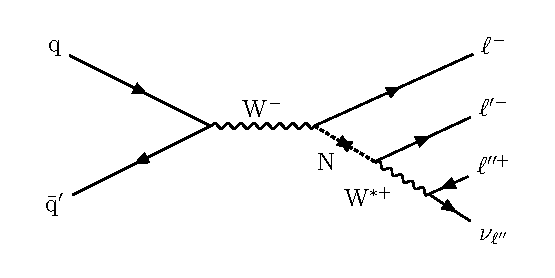
\includegraphics[width=0.45\textwidth]{Figures/c3/hnl_feyn.pdf}
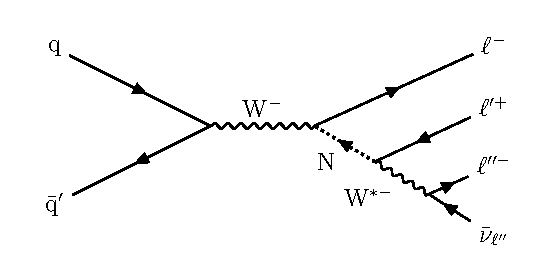
\includegraphics[width=0.45\textwidth]{Figures/c3/hnl_feyn_2.pdf}\\
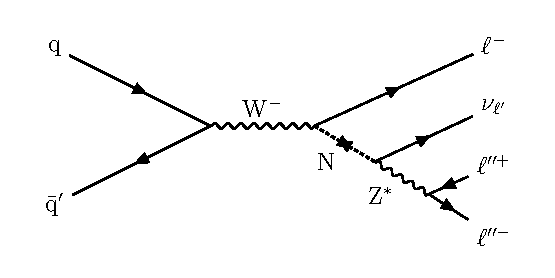
\includegraphics[width=0.45\textwidth]{Figures/c3/hnl_z_feyn.pdf}
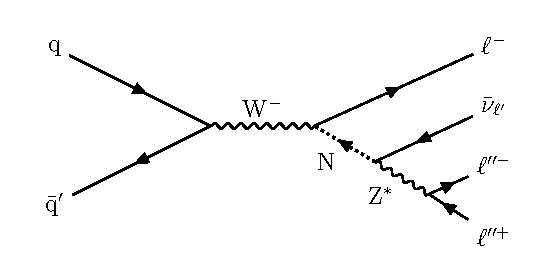
\includegraphics[width=0.45\textwidth]{Figures/c3/hnl_z_feyn_2.pdf}
\caption{Typical diagrams for the production of an HNL at the LHC 
($\hnl$) through its mixing with a SM neutrino, leading to a
final state with three charged leptons and a neutrino.
The HNL decay is mediated by either a $W$ (top row) or a $Z$ (bottom
row) boson.
In the diagrams on the left, $\hnl$ is assumed to be a Majorana
neutrino, thus $\ell$ and $\ell^\prime$ in the $W^\ast$-mediated
diagram (top) can have the same electric charge, with lepton-number
violation (LNV).
In the diagrams on the right instead, the $\hnl$ decay conserves the
lepton number (LNC) and can be either a Majorana or a Dirac
particle. Therefore $\ell$ and $\ell^\prime$ in the
$W^\ast$-mediated diagram (top right) have always opposite charge.
If \hnl couples exclusively to a single lepton-neutrino generation,
then $\ell$ and $\ell^\prime$ (or $\nu_{\ell^{\prime}}$) always belong
to the same lepton generation, and the lepton flavor is conserved
(LFC). If \hnl couples to multiple lepton families instead, then the
lepton flavor can be violated, $\ell\neq\ell^\prime$ (LFV).}
\label{fig:c3hnldiagram}
\end{figure}


\subsubsection{Decay width and branching ratio}\label{sec:decay_width}
The main consideration and difference between Majorana and Dirac HNL
is that in the first case the \hnl particle is defined as a particle
that is its own antiparticle. This implies that both $N_I\rightarrow
\PW^{+}\ell^-$, $\PZ\nu_{\ell}$, $H\nu_{\ell}$ and $N_I\rightarrow
\PW^{-}\ell^+$, $\PZ\bar{\nu}_{\ell}$, $H\bar{\nu}_{\ell}$ decay modes
are open. Assuming that the partial width of $N_I\rightarrow
\PW^{+}\ell^-$ and $N_I\rightarrow \PW^{-}\ell^+$ have the same
value, the total width for a Majorana neutrino and a Dirac
neutrino of same mass are related by:
\begin{equation}
\label{eq:width}
\Gamma^{Tot, \: Majorana}_{N_{I}} = 2 \times \Gamma^{Tot, \: Dirac}_{N_{I}}
\end{equation}
This leads to the following relationship between their lifetimes:
\begin{equation}
\label{eq:lifetime}
c\:\tau^{Tot, \: Majorana}_{N_{I}} = \frac{1}{2} \times c\:\tau^{Tot, \: Dirac}_{N_{I}}
\end{equation}

\subsection{Prompt and long-lived HNL}\label{sec:promptll}

The lifetime of a HNL is strongly dependent on $M_{N_I}$ and $|V_{\alpha I}|^2$,
and increases rapidly at small masses and low values of the mixing
parameter (see Fig.~\ref{fig:hnlLifetime}):
\begin{equation}
\label{eq:lifetimedependences}
c\:\tau_{N_{I}} \propto\mathrm{M_{N_I}^{-5}|V_{\alpha I}|^{-2}}
\end{equation}
As a consequence, the kinematics and acceptance of HNLs with masses
below about 20 GeV are significantly affected by their long lifetimes,
and must be accounted for in the signal simulation and in the resulting
interpretation.
If $\hnl$ has a long lifetime, in particular, its decay products
($\ell^{\pm\prime}$, $\ell^{\mp\prime\prime}$, $\nu_{\ell^{\prime\prime}}$ or
$\nu_{\ell^{\prime}}$, $\ell^{\pm\prime\prime}$, $\ell^{\mp\prime\prime}$, see Fig.~\ref{fig:c3hnldiagram})
emerge from a secondary vertex, spatially displaced with respect to
the primary vertex of the process, and distinguishable from it.
\begin{figure}
\centering
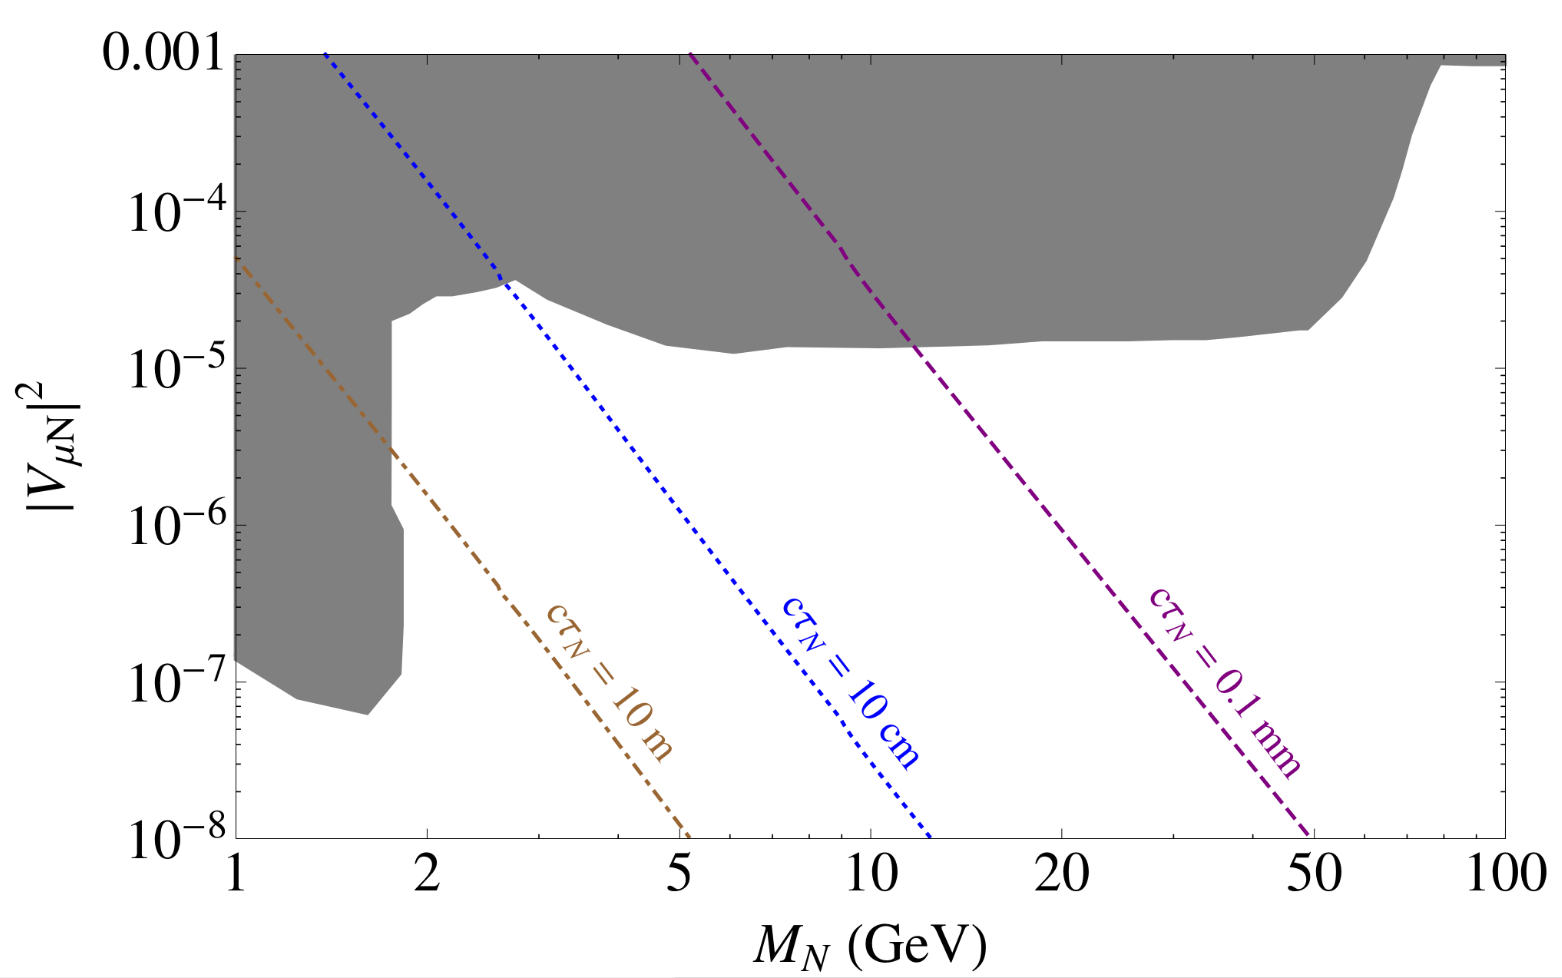
\includegraphics[width=0.78\textwidth]{Figures/c3/graph_displ.png}
\caption{The calculated lines for $c\tau$ of a HNL are shown as a function of its mass \mhnl
and its mixing parameter \mixpar to a single lepton family:
the three oblique lines correspond to $c\tau$ values of (from left to
right) 10~m,  10~cm, and 0.1~mm.
The shaded grey area represents---approximately---the region of the
parameter space excluded by previous searches.}
%% If $\hnl$ has a long lifetime, its decay products emerge from a
%% secondary vertex, distinguishable from the primary vertex of the
%% process.}
\label{fig:hnlLifetime}
\end{figure}


%%%%%%%%%%%%%%%%%%%%%%%%%%%%%%%%%%%%%%%%%%%%%%%%%%%%
%%%%%%%%%%%%%%%%%%%%%%%%%%%%%%%%%%%%%%%%%%%%%%%%%%%%
%%%%%%%%%%%%%%%%%%%%%%%%%%%%%%%%%%%%%%%%%%%%%%%%%%%%
\section{Theoretical and experimental constraints} \label{sec:currentlimits}
For a complete overview of the theoretical and experimental constraints of sterile neutrinos searches see References~\cite{Deppisch_2015,10.3389/fphy.2018.00040,PhysRevD.78.013010,Drewes_2017,DREWES2017250,Antusch_2014}.


Sterile neutrinos mix with $\nu_{SM}$, thus at small mixing the
active-neutrino mass states contain a small part of sterile
neutrinos. Consequently, the mass eigenstates of the HNLs couple to SM
neutrinos thanks to the tiny, but nonzero mixing $V_{\alpha sI}$, Eq.~\ref{eq:v2}.

In principle, in any weak processes where $\nu_{SM}$ participate, the
HNLs also do so. The strength is suppressed due to the smallness of
the $\nu_\alpha - N_I$ mixing angle,
but the production of a HNL in the interaction can manifest itself in the kinematic properties of the final decay products, because HNLs are much more massive than active neutrinos.
Therefore, it is possible to select particular channels and phase spaces that enhance some kinematic features associated to the presence of the sterile neutrino.

These properties are explored and exploited in the direct searches for HNLs.



\subsection{Direct HNL searches}\label{sec:c3directHNL}
Considering the wide theoretically accessible mass ranges (MeV-TeV) and taking into account
the several production and decay modes, we have a quite rich
experimental landscape. 
\begin{itemize}
\item For $M_N$ values below 1 MeV, HNL can be probed by
  neutrino-oscillation experiments~\cite{de_Gouv_a_2005};
\item for 10 eV $< M_N <$ 1 MeV, searches for neutrinoless double-beta decay,
  $0\nu\beta\beta$ and precision measurements of $\beta-$decay energy
  spectra have constrained the mixing \mixpare, only for Majorana cases~\cite{Deppisch_2015};
\item for 1 MeV $< M_N <$ 1 GeV, both \mixpare and \mixparm have been
  constrained by peak searches using leptonic decays of pions
  and kaons like $K \rightarrow \mu(e) N$, $\pi \rightarrow \mu(e)
  N$~\cite{Liventsev_2013};
\item for HNL in the MeV-GeV mass ranges, many searches through
  sterile neutrino decay products have been performed at beam-dump experiments~\cite{DORENBOSCH1986473};
\item for HNL in the GeV-TeV mass ranges, we enter the domain of
  the particle colliders.
\end{itemize}

Quite often the HNL bounds are shown in the 2D $V_{\alpha N} -
M_N$ plane for a specific mixing parameter V, under the assumption that all the other mixing angles are zero. 

To have a clear overview of the current experimental (and theoretical)
limits we can refer to
Figs.~\ref{fig:HNL_bc6_pbc_2},~\ref{fig:HNL_bc7_pbc_2}
and~\ref{fig:HNL_bc8_pbc_2}. Filled colored areas show the existing limits. For HNL masses below the charm mass, the limits are driven by the results from beam-dump experiments (PS191 and CHARM); for masses above
the charm mass, the most stringent limits are those coming from LEP experiments
(especially DELPHI), from Belle, and, more recently, from CMS and ATLAS.



\begin{figure}[h]
  \centering
  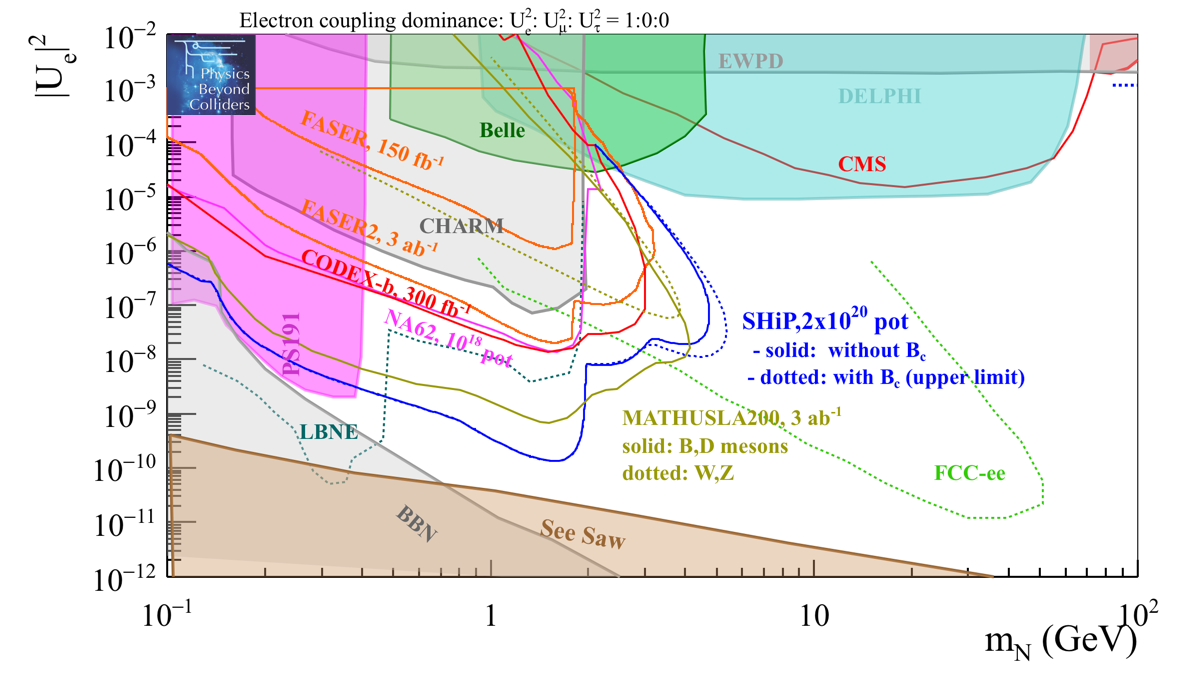
\includegraphics[width=.90\textwidth]{Figures/c3/HNL_bc6_pbc_2.png}
    \caption{Sensitivity to HNL with coupling to $\nu_e$ only. Current bounds (filled areas) and 10-15 years prospects for projects
(SHiP, MATHUSLA200, CODEX-b and FASER2) (solid lines). Projections for a LBNE
near detector with $5\times 10^{21}$ protons-on-target and from FCC-ee with
$10^{12}$ $\PZ_0$ decays are also shown.
The gray contour named "BBN'' corresponds to a HNL lifetime $>1$sec,
which is disfavored by BBN~\cite{Ruchayskiy_2012}. The brown line
labeled "seesaw'' represents the scale of mixing in general expected
in the canonical seesaw. The very light gray at the top
labeled as "EWPD'' is the 90\% C.L. exclusion limit from the
electroweak precision data~\cite{Antusch_2015}. The other solid
contours are explained in the text. 
% The green contour labeled "Belle'' is the exclusion
%region at 90\% C.L from HNL searches in B-meson decays at
%Belle~\cite{Liventsev_2013}. Those labeled "PS191'' (magenta) and
%"CHARM' (gray) are excluded at 90\% C.L. from beam-dump experiments.
}
  \label{fig:HNL_bc6_pbc_2}
\end{figure}

\begin{figure}[h]
  \centering
  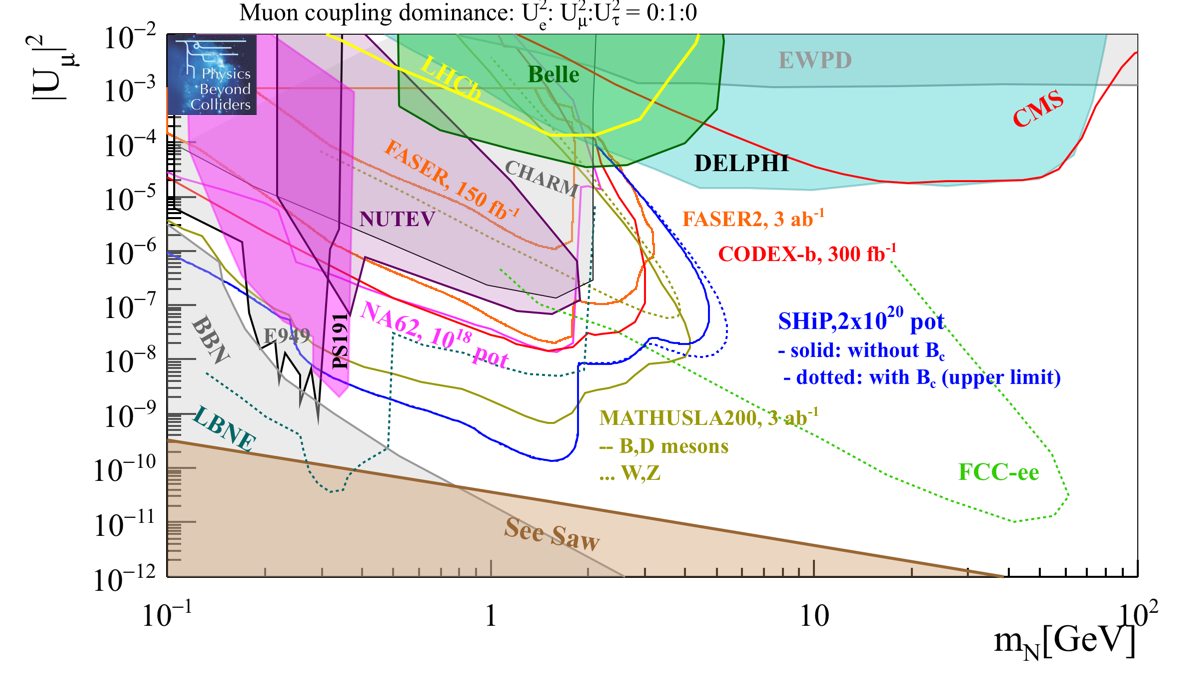
\includegraphics[width=.90\textwidth]{Figures/c3/HNL_bc7_pbc_2.png}
    \caption{Sensitivity to HNL with coupling to $\nu_\mu$ only. Current bounds (filled areas) and 10-15 years prospects for projects
(SHiP, MATHUSLA200, CODEX-b and FASER2) (solid lines). Projections for a LBNE
near detector with $5\times 10^{21}$ protons-on-target and from FCC-ee with $10^{12}$ $\PZ_0$ decays are also shown. The gray contour named "BBN'' corresponds to a HNL lifetime $>1$sec,
which is disfavored by BBN~\cite{Ruchayskiy_2012}. The brown line
labeled "seesaw'' represents the scale of mixing in general expected
in the canonical seesaw. The very light gray at the top
labeled as "EWPD'' is the 90\% C.L. exclusion limit from the
electroweak precision data~\cite{Antusch_2015}. The other solid
contours are explained in the text.}
  \label{fig:HNL_bc7_pbc_2}
\end{figure}

\begin{figure}[h]
  \centering
  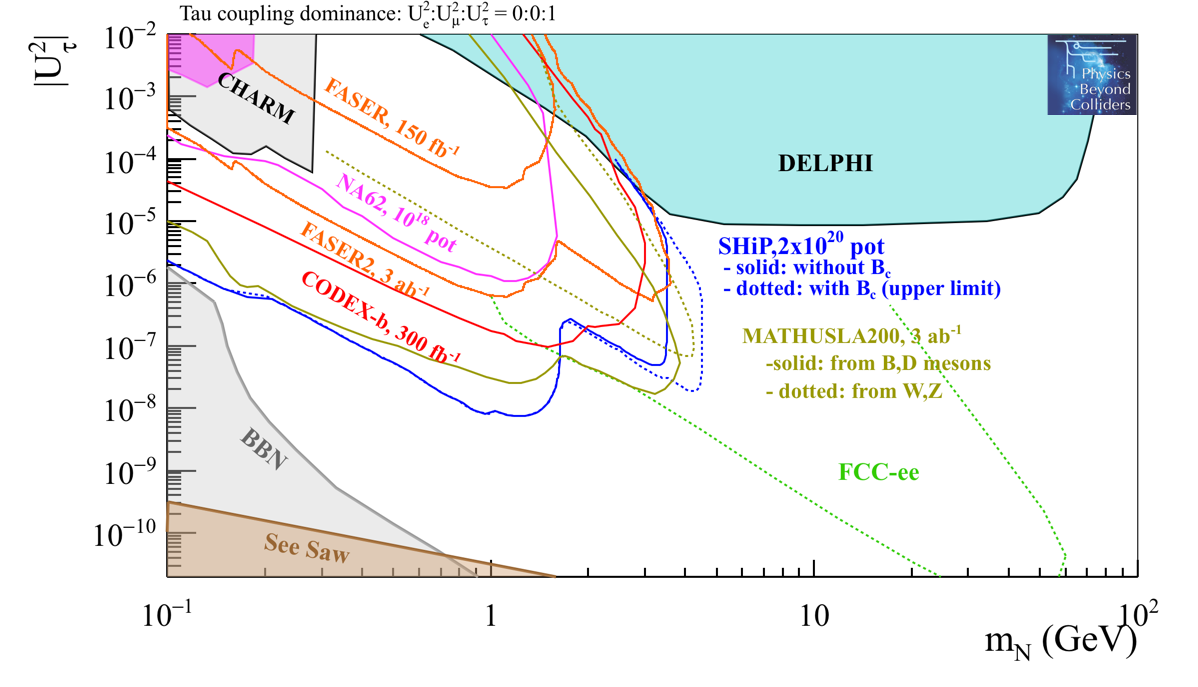
\includegraphics[width=.90\textwidth]{Figures/c3/HNL_bc8_pbc_2.png}
    \caption{Sensitivity to HNLs with coupling to $\nu_\tau$ only. Current bounds (filled areas) and 10-15 years prospects for projects
(SHiP, MATHUSLA200, CODEX-b and FASER2) (solid lines). Projections from FCC-ee with $10^{12}$ $\PZ_0$ decays are also shown.}
  \label{fig:HNL_bc8_pbc_2}
\end{figure}

A brief experiment-focused overview follows:
\begin{itemize}
\item \textbf{PS191} (CERN, PS Beam 1983)~\cite{BERNARDI1988332}: the PS191
  experiment was specifically designed to look for neutrino decays in
  low-energy neutrino beams. It was a detector composed of a 12 m long
  decay volume followed by a fine-grain calorimeter. No sterile
  neutrino candidates were observed but the analysis of neutrino
  interactions in the calorimeter shows a possible excess of events
  with electrons~\cite{Vannucci:1985vs}.
\item \textbf{CHARM} (CERN, SPS beam 1985)~\cite{DORENBOSCH1986473}: a search
  for HNL decays  was performed by the CHARM Collaboration using a
  neutrino beam produced by dumping 400 GeV protons on a thick Copper
  target and looking for possible visible decays. The sterile neutrino was assumed to be produced in charmed D meson decays, \ie $c\rightarrow s W^{*}$ with $W^{*} \rightarrow \ell \hnl$. The following decays were considered, \hnl $\rightarrow
  e^+e^-\nu_e$, $\rightarrow \mu^+e^-\nu_\mu$ and $\rightarrow
  \mu^+\mu^-\nu_\mu$ and the limits were set on \mixpare and
  \mixparm $< \:10^{-7}$ for \hnl masses around 1.5 GeV. 
\item \textbf{Belle} (KEK, asymmetric-energy $e^+e^-$ collider, 2012)~\cite{Liventsev_2013}: the Belle Collaboration
  performed a search for heavy neutral leptons in B-meson
  decays. The data sample contained $772\times 10^6$ $B\overline{B}$
  pairs collected at the $\Upsilon(4S)$ resonance. The limits
  on the mixing parameter were obtained analyzing the $B\overline{B}$ pairs
  events using the leptonic and semileptonic B meson decay,
  $B\rightarrow X\ell\nu_R$, where $\ell = e, \: \mu$ and the $X$ was
  either a charmed D meson, a light meson ($\pi, \: \rho, \: \eta$) or
  nothing (leptonic decay). Upper limits were set on \mixpare and
  \mixparm in the mass range 0.5--5.0 GeV. 
\item \textbf{DELPHI} (CERN, lepton collider LEP, 1997)~\cite{Abreu:1996pa}:
  up to the publication of the results presented in this thesis, the most stringent limits between 1 GeV and 10 GeV have been those published by the DELPHI Collaboration. HNL searches were performed
  using the data collected by DELPHI, corresponding to $3.3
  \times 10^6$ hadronic $Z_0$ decays at LEP1. This set of results is, up to
  this day, one of the most complete, including both the short-lived HNL and the long-lived
  HNL scenario and all three lepton flavor couplings. 
  According to the mass and lifetime ranges of the HNL, four separate searches were performed, two for short-lived \hnl production giving monojet or acollinear jet topologies, 
  and two for long-lived \hnl looking for detectable secondary vertices or calorimeter clusters.
 Upper limits were set for the branching ratio $BR (\: Z_0\rightarrow$ \hnl) of
 about $1.3 \times 10^{-6}$ at 95\% C.L. for \hnl masses between 1 and
 80\GeV. An additional combination of the short and long lived HNL searches was performed providing the upper limits on \mixpar for \hnl masses between 3.5 and
 50\GeV. 
\item \textbf{CMS and ATLAS} (CERN, LHC pp beam, 2019): there have been several searches for HNLs in both CMS and ATLAS.
The ATLAS experiment recently reported on a search for HNLs using events with three charged leptons~\cite{atlasintro2} using 
pp collisions data corresponding to integrated luminosities of 32.9 to
36.1 $fb^{-1}$. 
The search is performed in channels with three muons or two muons plus
one electron---providing sensitivity  to \mixparm only---, where the 
displaced decay vertex of the HNL was exploited.
CMS performed searches for HNLs only using prompt leptons,
either in final states with two same-charge leptons and one or two jets
(\(\PW^{\pm(\ast)}\to\ell^{\pm}\hnl\to\ell^{\pm}\ell^{\prime\pm}q\bar{q}^{\prime}\))~\cite{Sirunyan:2018xiv},
or in final states with three prompt leptons and \ptmiss 
in a mass range of 20 GeV to 1.7 TeV.
CMS searches with three charged leptons in the final state using the leptonic \PW decay are going to be extensively discussed in this
dissertation.
\end{itemize}

\subsection{Theoretical constraints on HNL}
In the following list, we tried so summarize the current constraints
coming from theoretical predictions and from the most recent results (Figs.~\ref{fig:HNL_bc6_pbc_2},~\ref{fig:HNL_bc7_pbc_2}
and~\ref{fig:HNL_bc8_pbc_2}.)
\begin{itemize}
\item \textbf{Searches for Charged Lepton Flavor Violation}. If we consider a HNL with a
  mass close to the EW scale and with large off-diagonal Yukawa couplings,
  then this can lead to LFV in decays of charged leptons. Thus,
  testing LFV in multi-lepton searches could be an indirect way to
  probe the existence of HNL. Searches for such processes have
  placed 90\% C.L. upper limits on decay branching rates, \ie
  $BR(\mu^+\rightarrow e^+\gamma) < 4.2\times 10^{-13}$,
  $BR(\mu^+\rightarrow e^+e^+e^-) < 1.0\times 10^{-12}$ and
  $BR(\tau^-\rightarrow e^-\mu^+\mu^-) < 2.7\times 10^{-8}$. For a 
  complete summary and references see~\cite{Pascoli_2019}.
\item \textbf{Cosmological constraints on light neutrino masses}. The Planck
  Satellite's measurements of the large scale structures in the
  universe, combined with the WMAP + highL + BAO data, have set the
  upper limits on the sum of all the light
  neutrinos~\cite{Aghanim:2018eyx}.
\begin{equation}
\label{eq:summasses}
\sum_{m} m_{\nu_m} < 0.12 \: eV, \;\;\;\; at \;95\% \: C.L.
\end{equation}
This upper limit on the active neutrino masses is directly connected
with the possibility of the existence of HNLs and with the predicted
numbers of \hnl, $\mathcal{N}$.
If the seesaw mechanism is assumed to be responsible for the origin of neutrino masses,
one RH neutrino is necessary per observed nonzero light
neutrino mass~\cite{Alekhin_2016}.
To conclude, the interpretation of direct search experiments limits and cosmological constraint both strongly
depend on $\mathcal{N}$ and the $\nu_{SM}$
mass~\cite{DREWES2017250,drewes2015theoretical}. To clarify, for
$\mathcal{N}=3$, if the lightest neutrino is massless, no
lower bound on the mixing parameter \mixpar can be set.
On the other hand, if it is the case like in Eq.~\ref{eq:summasses}, then there is a lower
bound on \mixpar~\cite{DREWES2017250}.
\item \textbf{BBN constraints}. Observing
  Figs.~\ref{fig:HNL_bc6_pbc_2},~\ref{fig:HNL_bc7_pbc_2}
  and~\ref{fig:HNL_bc8_pbc_2}, a HNL that falls on the left of the
  Big Bang Nucleosynthesis line would live long enough in
  the early universe to cause an overproduction of primordial
  Helium-4~\cite{Ruchayskiy_2012}.
\item \textbf{Seesaw limit}. Below the line of the seesaw limit, the
  mixing of the sterile neutrinos with the active ones becomes too
  weak to be able to produce the pattern of neutrino flavor oscillations that has been observed~\cite{Canetti_2010}. 
\end{itemize}

\section{Summary}
In this chapter we illustrate the relevance and the interest for the
current HNL search program, describing first the theory setting of RH
neutrinos and then reporting the rich plethora of experiments and results
focusing on HNL.\\
In the SM, all the fermions are known to have both
left- and right-handed chirality, the only exception comes from the
neutrinos. One argument in favor of the introduction of massive RH
neutrinos is that they give an answer to the SM problem of the
neutrino masses via a type-I seesaw mechanism. The massless neutrino
problem is one of the open questions in physics that indicates that
other fundamental physics remains to be unmasked.

When we hypothesize a new particle as RH neutrinos, $N_{I}$, we
are interested in their properties like the mass $M_I$ of the HNLs and
their mixing parameter, $|V_{\alpha I}|^2$  with the SM neutrino of flavor $\alpha$,
controlled by the Yukawa coupling $F_{\alpha I}$. The values of $|V_{I
  \alpha}|^2$ is unknown and usually the experimental
sensitivity is expressed in terms of the coupling $|V_{\alpha I}|^2$
($= |F_{\alpha I}|^2$) as a function of $M_I$ for a given flavor
$\alpha$.

A list of direct HNL search results is presented; we give an overview
of the experimental current and past landscape describing the different decay modes and
mass ranges that are targeted by the single measurement.
The strategies in direct HNL searches depends greatly on the mass
which we desire investigating. For $M_{I} > 5$\GeV, \hnl can be
produced uniquely at either LHC or at similar energy colliders, via a few
mechanisms (vector boson fusion, s-channel exchange of virtual
W-bosons or in real gauge boson decays) according to the production
energy and \hnl mass. Extensive explanation is given in the following
Chapter~\ref{Chapter4}. For $M_{I} < 5$\GeV, we recur to b-factories
or fixed target experiments. \\
In this chapter, special attention is paid to lepton and hadron collider
searches. The LEP results from DELPHI happen to be the best results at
low mass from collider experiment up to the publication of the results
of this dissertation. For the author, the outstanding sensitivity al low mass from
$e^{+}e^{-}$ data was surely a good motivation to invest a quite
important effort to extend as well the low mass sensitivity of
the CMS experiment. Chronologically I have focused first in the
moderate and high mass search to migrate to very low mass search which
necessarily requires the inclusion of displaced scenarios.

Additionally it is presented an overview of the theoretical HNL
constraints.

Taking into account 
the current experimental and theoretical limits on the HNL
mass, we described the allowed mass window of sixteen orders of magnitude
$100\ \MeV < M_{I} < 1015\ \TeV$. The summary of the HNL constrains is shown in
Figure~\ref{fig:marcoscheme}. 

\begin{figure}[h!]
  \centering
  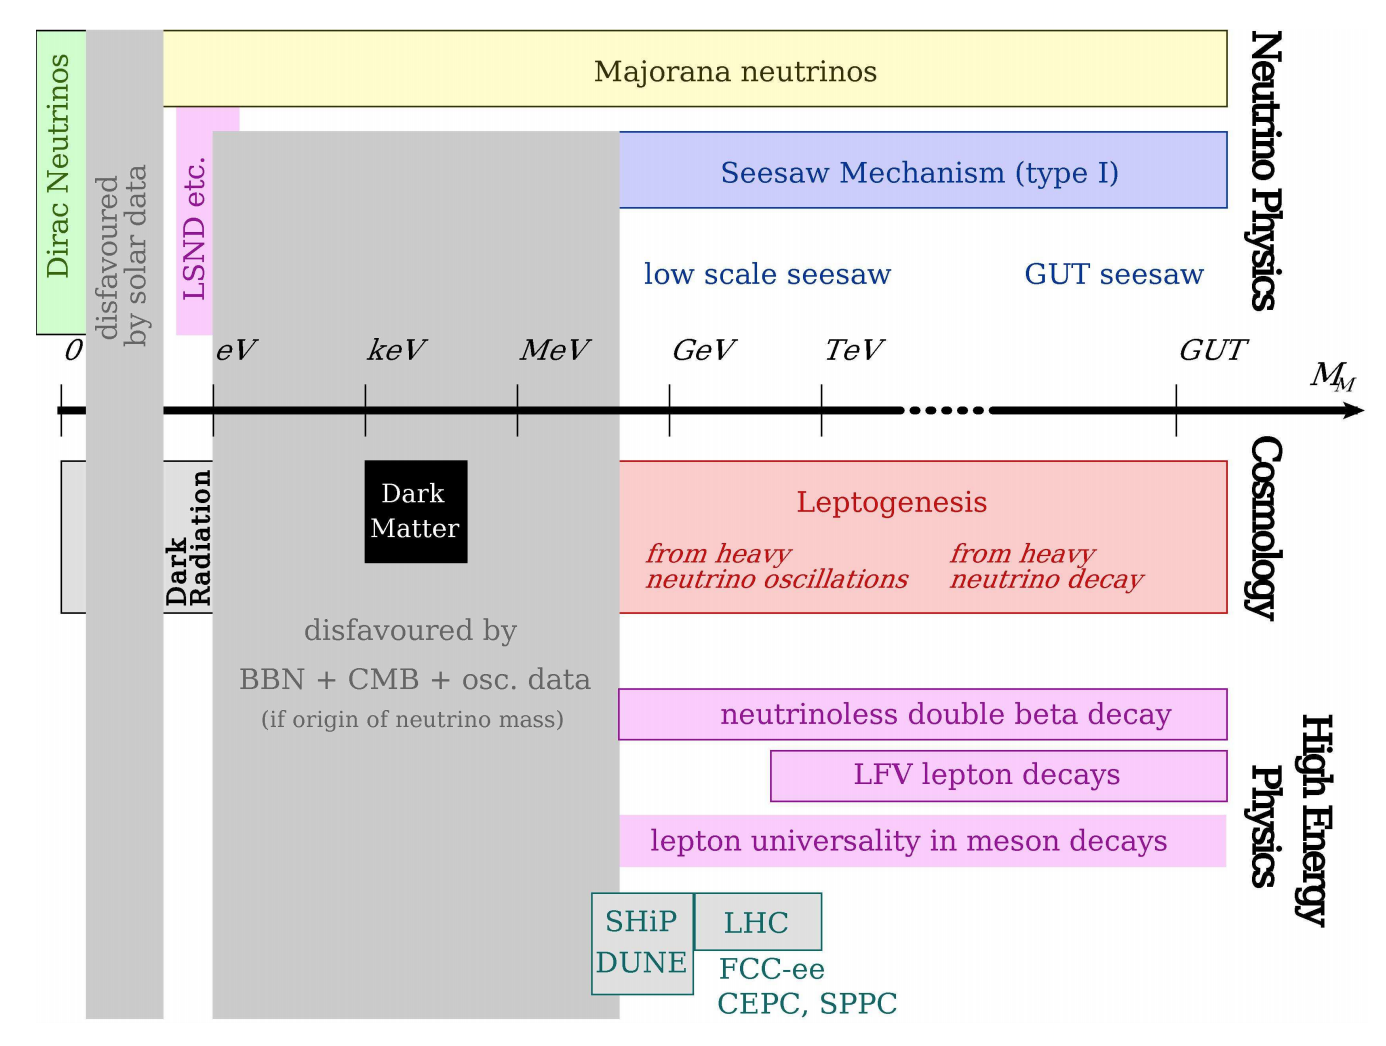
\includegraphics[width=.79\textwidth]{Figures/c3/marcoscheme.png}
    \caption{A schematic overview from Reference~\cite{DREWES2017250} ``of the allowed range of values for the “seesaw scale” and their implications for neutrino physics, cosmology and high
energy physics''.~\cite{DREWES2017250}}
  \label{fig:marcoscheme}
\end{figure}










\clearpage

